\documentclass[a4paper,12pt]{article}
\usepackage{ctex}
\usepackage{graphicx}
\usepackage{hyperref}
\usepackage{geometry}
\usepackage{xcolor}
\usepackage{listings}
\usepackage{booktabs}
\usepackage{enumitem}
\usepackage{fancyhdr}
\usepackage{longtable}
\usepackage{float}

\geometry{a4paper,left=2.5cm,right=2.5cm,top=2.5cm,bottom=2.5cm}

\hypersetup{
    colorlinks=true,
    linkcolor=blue,
    filecolor=magenta,      
    urlcolor=cyan,
    pdftitle={需求分析规格说明文档},
    pdfpagemode=FullScreen,
}

\lstset{
    basicstyle=\ttfamily\small,
    breaklines=true,
    frame=single,
    xleftmargin=15pt,
    xrightmargin=15pt,
    backgroundcolor=\color{gray!10}
}

\title{需求分析规格说明文档}
\author{项目组}
\date{\today}

\pagestyle{fancy}
\fancyhf{}
\fancyhead[L]{需求分析规格说明文档}
\fancyhead[R]{\thepage}
\fancyfoot[C]{项目文档}

\begin{document}

\maketitle
\tableofcontents
\newpage

\section{文档概述}

\subsection{文档目的}

本文档是项目的需求分析规格说明文档,旨在详细描述系统的功能需求、非功能需求、用例分析和各模块交互关系,作为后续设计和开发工作的基础依据。它明确定义了用户需求,并将这些需求转化为可实现的技术规范。同时,通过用例图描述System组在项目中的职责和与其他组(UI组、Data组和Analysis组)的交互关系,为项目各方提供清晰的职责界定和协作指南。

\subsection{项目背景}

本项目旨在开发一个综合性系统,由四个主要组成部分协同工作:系统组(System)、用户界面组(UI)、数据组(Data)和分析组(Analysis)。这四个组各司其职,共同构建一个完整的解决方案,以满足用户的需求和业务目标。系统组作为项目的技术基础设施提供者,是项目技术架构的设计者和实现者,负责系统核心功能的开发。

\subsection{读者对象}

本文档适用于以下读者:
\begin{itemize}
  \item 项目管理人员:了解项目整体需求和范围
  \item 开发团队成员:理解具体技术需求和实现细节
  \item 测试人员:制定测试计划和用例
  \item 用户代表:确认系统是否满足业务需求
\end{itemize}

\subsection{参考文献}

\begin{enumerate}
  \item Claude 3.7
  \item QwQ
\end{enumerate}

\section{系统概述}

\subsection{系统目标}

本系统旨在[此处描述系统的主要目标和要解决的问题]。
通过整合用户界面、系统架构、数据处理和分析功能,为用户提供全面的解决方案,提高工作效率和决策质量。

\subsection{系统范围}

本系统包括但不限于以下功能范围:
\begin{itemize}
  \item 用户界面展示和交互
  \item 系统核心架构和服务
  \item 数据采集、存储和管理
  \item 数据分析和可视化
\end{itemize}

\subsection{系统架构概述}

系统由四个主要组件构成,各组件职责如下:

\begin{itemize}
  \item \textbf{系统组(System)}:负责核心架构设计、API实现、第三方服务集成、系统部署、性能优化、安全保障及监控系统
  \item \textbf{用户界面组(UI)}:负责用户界面设计和实现、用户体验优化、前端与后端API交互
  \item \textbf{数据组(Data)}:负责数据模型设计、数据库实现、数据处理流程、数据质量保障
  \item \textbf{分析组(Analysis)}:负责数据分析算法、报表生成、数据可视化、决策支持模型
\end{itemize}

各组件之间通过定义良好的接口进行交互,如下图所示:

\begin{figure}[H]
    \centering
    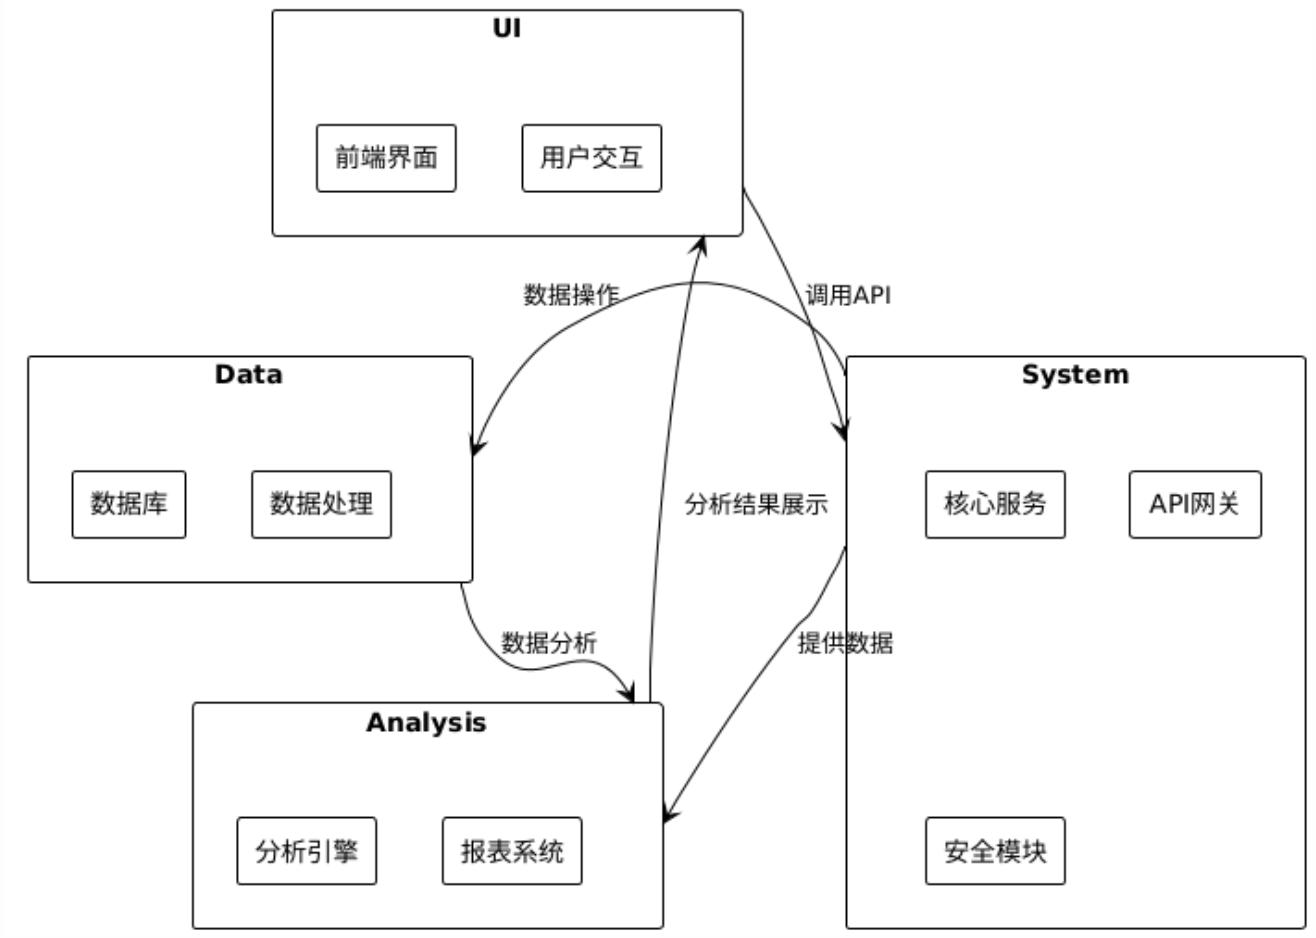
\includegraphics[width=0.75\linewidth]{assets/7.png}
    \caption{系统架构概述图}
    \label{fig:system-architecture}
\end{figure}

\section{用户需求}

\subsection{用户角色定义}

系统识别了以下主要用户角色:

\begin{enumerate}
  \item \textbf{系统管理员}:负责系统管理和维护
  \item \textbf{普通用户}:使用系统的主要功能
  \item \textbf{分析师}:进行数据分析和报表生成
  \item \textbf{数据管理员}:管理系统数据和权限
\end{enumerate}

\subsection{用户场景}

以下是主要用户场景的概述:

\begin{enumerate}
  \item 用户登录与认证
  \item 数据录入与编辑
  \item 数据查询与检索
  \item 数据分析与报表生成
  \item 系统管理与配置
  \item 安全审计与监控
\end{enumerate}

\section{功能需求}

\subsection{UI组功能需求}

\begin{enumerate}
  \item \textbf{用户界面设计}
  \begin{itemize}
    \item 设计符合用户体验原则的界面布局
    \item 实现响应式设计,适配不同设备
    \item 提供统一的视觉风格和组件库
  \end{itemize}
  
  \item \textbf{用户交互实现}
  \begin{itemize}
    \item 实现用户登录、注册、密码重置等基础功能
    \item 提供个性化设置和主题定制
    \item 实现多语言支持
  \end{itemize}
  
  \item \textbf{前端数据展示}
  \begin{itemize}
    \item 实现数据表格、图表等展示组件
    \item 提供数据筛选、排序和分页功能
    \item 支持数据导出和打印
  \end{itemize}
\end{enumerate}

\subsection{System组功能需求}

System组在项目中的主要职责是作为技术基础设施提供者,负责系统核心功能的开发。以下是System组的具体功能需求:

\begin{enumerate}
  \item \textbf{构建部署流程}
  
  \begin{figure}[H]
    \centering
    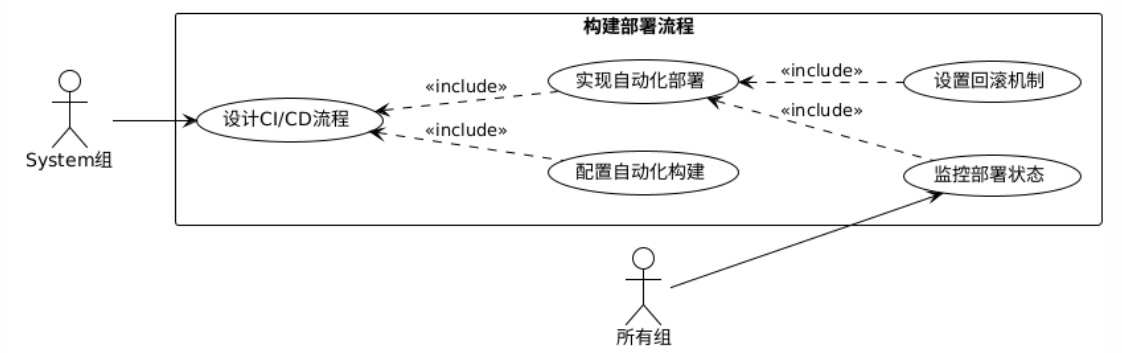
\includegraphics[width=0.75\linewidth]{assets/image1.png}
    \caption{构建部署流程用例图}
    \label{fig:deployment-process}
  \end{figure}
  
  \begin{itemize}
    \item 设计并实现完整的CI/CD流程
    \item 配置自动化构建和测试环境
    \item 提供部署状态监控
    \item 建立部署失败的回滚机制
  \end{itemize}
  
  \item \textbf{集成第三方服务}
  
  \begin{figure}[H]
    \centering
    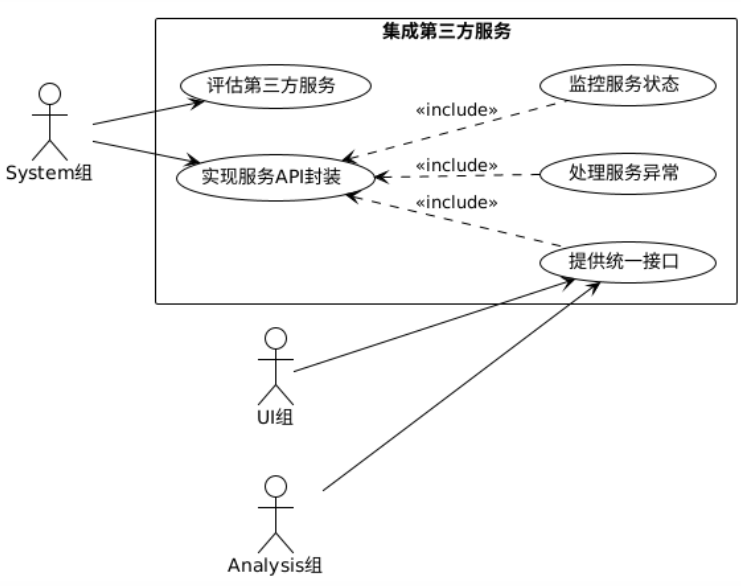
\includegraphics[width=0.75\linewidth]{assets/image11.png}
    \caption{集成第三方服务用例图}
    \label{fig:third-party-services}
  \end{figure}
  
  \begin{itemize}
    \item 评估和选择适合项目需求的第三方服务
    \item 实现对第三方API的封装
    \item 提供统一的接口规范
    \item 处理第三方服务异常情况
    \item 监控第三方服务的可用性和性能
  \end{itemize}
  
  \item \textbf{协同开发数据库}
  
  \begin{figure}[H]
    \centering
    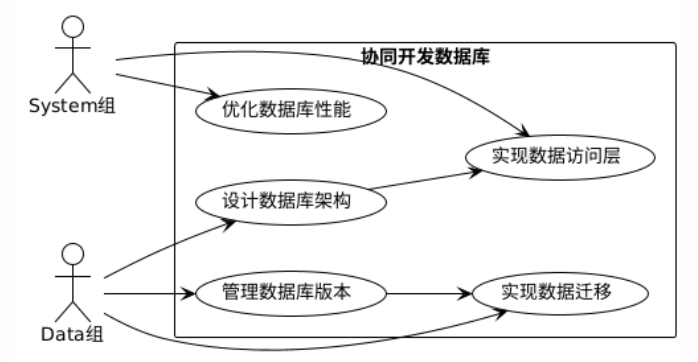
\includegraphics[width=0.75\linewidth]{assets/image8.png}
    \caption{协同开发数据库用例图}
    \label{fig:database-development}
  \end{figure}
  
  \begin{itemize}
    \item 与Data组协作实现数据访问层
    \item 优化数据库性能
    \item 实现数据缓存机制
  \end{itemize}
  
  \item \textbf{API设计与实现}
  
  \begin{figure}[H]
    \centering
    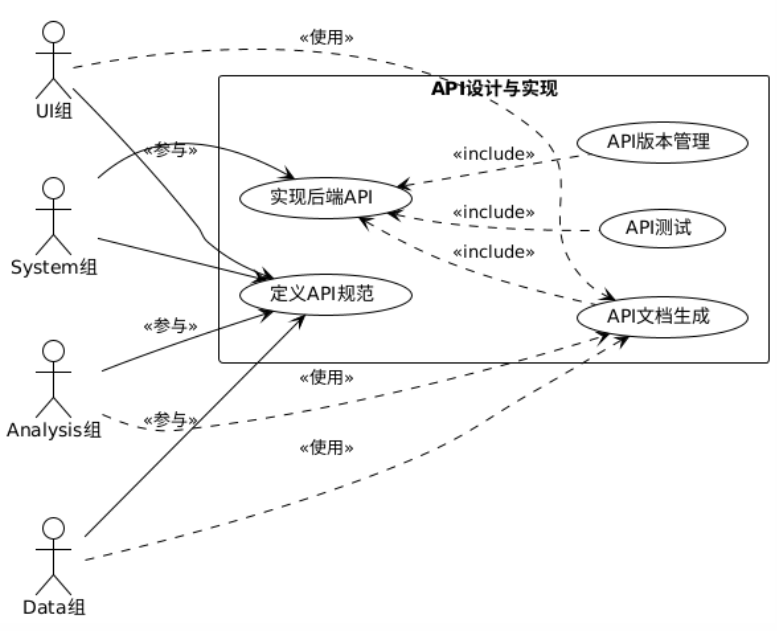
\includegraphics[width=0.75\linewidth]{assets/image4.png}
    \caption{API设计与实现用例图}
    \label{fig:api-design}
  \end{figure}
  
  \begin{itemize}
    \item 制定API设计规范和标准
    \item 实现所有后端API功能
    \item 生成完整的API文档
    \item 进行API单元测试和集成测试
    \item 管理API版本和兼容性
  \end{itemize}
  
  \item \textbf{性能优化}
  
  \begin{figure}[H]
    \centering
    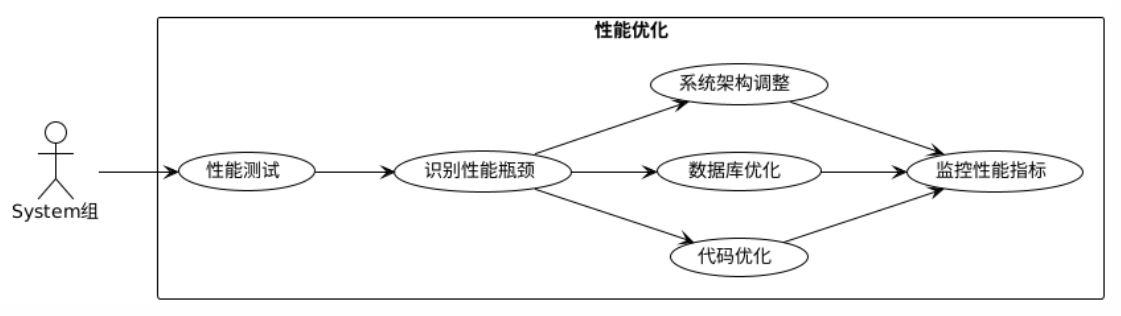
\includegraphics[width=0.75\linewidth]{assets/image5.png}
    \caption{性能优化用例图}
    \label{fig:performance-optimization}
  \end{figure}
  
  \begin{itemize}
    \item 设计并执行性能测试方案
    \item 分析并识别系统性能瓶颈
    \item 优化代码执行效率
    \item 与Data组协作进行数据库性能优化
    \item 必要时进行系统架构调整
    \item 持续监控系统性能指标
  \end{itemize}
  
  \item \textbf{安全保障}
  
  \begin{figure}[H]
    \centering
    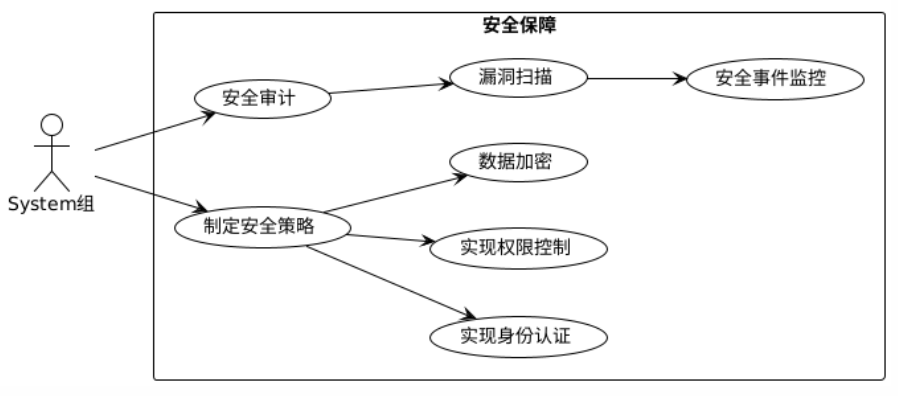
\includegraphics[width=0.75\linewidth]{assets/image6.png}
    \caption{安全保障用例图}
    \label{fig:security-protection}
  \end{figure}
  
  \begin{itemize}
    \item 制定系统安全策略和标准
    \item 实现身份认证和授权机制
    \item 实现细粒度的权限控制
    \item 敏感数据加密存储和传输
    \item 防止常见安全威胁(SQL注入、XSS等)
    \item 定期进行安全审计和漏洞扫描
    \item 实施安全事件监控和响应机制
  \end{itemize}
  
  \item \textbf{监控与日志系统}
  
  \begin{figure}[H]
    \centering
    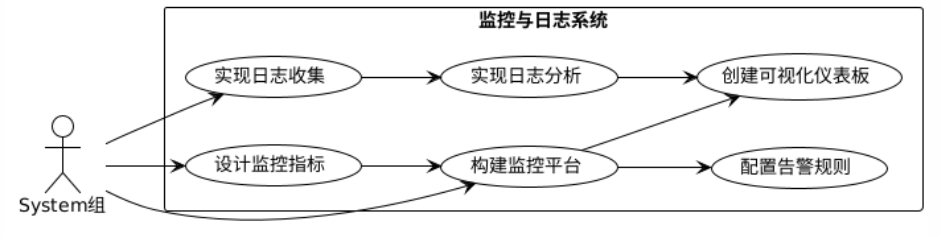
\includegraphics[width=0.75\linewidth]{assets/image7.png}
    \caption{监控与日志系统用例图}
    \label{fig:monitoring-logging}
  \end{figure}
  
  \begin{itemize}
    \item 设计系统关键监控指标
    \item 实现全面的日志收集机制
    \item 构建统一的监控平台
    \item 配置合理的告警规则
    \item 实现日志聚合和分析功能
    \item 创建直观的可视化仪表板
  \end{itemize}
\end{enumerate}

\subsection{Data组功能需求}

\begin{enumerate}
  \item \textbf{数据库设计}
  \begin{itemize}
    \item 设计数据库模型和表结构
    \item 定义数据约束和关系
    \item 实现数据版本控制
  \end{itemize}
  
  \item \textbf{数据处理流程}
  \begin{itemize}
    \item 实现数据ETL(提取、转换、加载)流程
    \item 提供数据批量导入和导出功能
    \item 实现数据清洗和验证机制
  \end{itemize}
  
  \item \textbf{数据质量管理}
  \begin{itemize}
    \item 实现数据质量检查规则
    \item 监控数据完整性和一致性
    \item 提供数据修复工具
  \end{itemize}
\end{enumerate}

\subsection{Analysis组功能需求}

\begin{enumerate}
  \item \textbf{数据分析算法}
  \begin{itemize}
    \item 实现统计分析功能
    \item 提供预测分析模型
    \item 支持自定义分析规则
  \end{itemize}
  
  \item \textbf{报表生成}
  \begin{itemize}
    \item 设计标准报表模板
    \item 支持自定义报表
    \item 实现报表定时生成和分发
  \end{itemize}
  
  \item \textbf{数据可视化}
  \begin{itemize}
    \item 提供多种图表和可视化组件
    \item 支持交互式数据探索
    \item 实现数据钻取和聚合分析
  \end{itemize}
\end{enumerate}

\section{非功能需求}

\subsection{性能需求}

\begin{enumerate}
  \item \textbf{响应时间}
  \begin{itemize}
    \item 页面加载时间不超过3秒
    \item API接口响应时间不超过1秒
    \item 报表生成时间不超过5秒
  \end{itemize}
  
  \item \textbf{并发处理}
  \begin{itemize}
    \item 系统支持至少100个并发用户
    \item 数据库能同时处理50个并发事务
  \end{itemize}
  
\end{enumerate}

\subsection{可靠性需求}

\begin{enumerate}
  
  \item \textbf{数据备份与恢复}
  \begin{itemize}
    \item 每日进行数据备份
    \item 数据恢复时间不超过4小时
  \end{itemize}
  
  \item \textbf{错误处理}
  \begin{itemize}
    \item 系统提供明确的错误提示
    \item 关键操作提供回滚机制
  \end{itemize}
\end{enumerate}

\subsection{安全需求}

\begin{enumerate}
  \item \textbf{身份认证与授权}
  \begin{itemize}
    \item 实现多因素认证
    \item 基于角色的访问控制
    \item 定期密码更新策略
  \end{itemize}
  
  \item \textbf{数据安全}
  \begin{itemize}
    \item 敏感数据加密存储
    \item 通信加密(HTTPS)
  \end{itemize}
  
\end{enumerate}

\subsection{可维护性需求}

\begin{enumerate}
  \item \textbf{模块化设计}
  \begin{itemize}
    \item 系统采用松耦合、高内聚的设计原则
    \item 支持模块独立更新和部署
  \end{itemize}
  
  \item \textbf{文档完备}
  \begin{itemize}
    \item 提供详细的系统架构文档
    \item 编写完整的API文档
    \item 维护代码注释和关键算法说明
  \end{itemize}
  
  \item \textbf{可测试性}
  \begin{itemize}
    \item 支持自动化单元测试和集成测试
    \item 提供测试环境和测试数据
  \end{itemize}
\end{enumerate}

\section{用例分析}

\subsection{系统组用例总览}

以下用例图展示了System组的主要职责和与其他组的交互关系:

\begin{figure}[H]
    \centering
    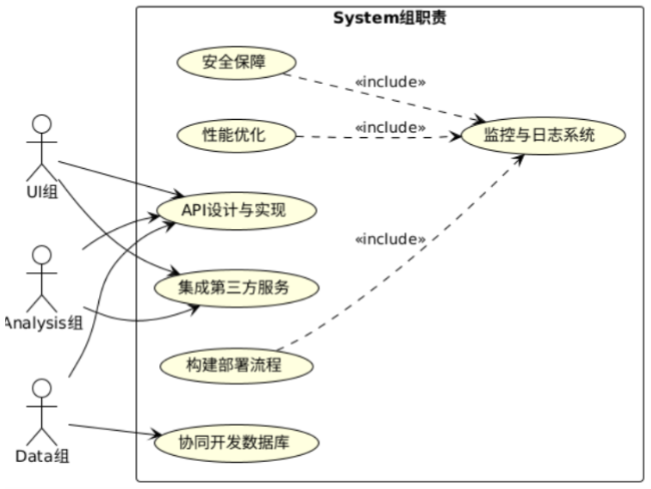
\includegraphics[width=0.75\linewidth]{assets/image2.png}
    \caption{系统组用例总览图}
    \label{fig:system-overview}
\end{figure}

\subsection{系统组用例分析}

\subsubsection{构建部署流程}

\textbf{用例名称}:构建部署流程

\textbf{行为主体}:System组

\textbf{前置条件}:
\begin{itemize}
  \item 项目代码仓库已建立
  \item 部署环境已准备就绪
\end{itemize}

\textbf{后置条件}:
\begin{itemize}
  \item 自动化CI/CD流程可正常运行
  \item 各组可使用部署流程部署代码
\end{itemize}

\textbf{基本流程}:
\begin{enumerate}
  \item System组设计CI/CD流程
  \item 配置自动化构建环境
  \item 实现自动化部署机制
  \item 设置部署监控和回滚机制
  \item 各组使用部署流程部署代码
\end{enumerate}

\textbf{替代流程}:
\begin{enumerate}
  \item 部署失败时,自动触发回滚机制
  \item 环境不可用时,提供手动部署选项
\end{enumerate}

\textbf{交付物}:
\begin{itemize}
  \item CI/CD配置文件
  \item 部署脚本
  \item 部署文档
\end{itemize}

\subsubsection{集成第三方服务}

\textbf{用例名称}:集成第三方服务

\textbf{行为主体}:System组

\textbf{前置条件}:
\begin{itemize}
  \item 已确定需要集成的第三方服务
  \item 已获取相关API文档和访问权限
\end{itemize}

\textbf{后置条件}:
\begin{itemize}
  \item 第三方服务成功集成到系统中
  \item 提供统一的接口供其他组使用
\end{itemize}

\textbf{基本流程}:
\begin{enumerate}
  \item 评估和选择适合项目需求的第三方服务
  \item 实现对第三方API的封装
  \item 提供统一的接口规范
  \item 处理第三方服务异常情况
  \item 监控第三方服务的可用性和性能
\end{enumerate}

\textbf{替代流程}:
\begin{enumerate}
  \item 第三方服务不可用时,提供降级策略
  \item 接口变更时,提供兼容性处理
\end{enumerate}

\textbf{交付物}:
\begin{itemize}
  \item 第三方服务集成文档
  \item API封装代码
  \item 服务配置指南
\end{itemize}

\subsubsection{协同开发数据库}

\textbf{用例名称}:协同开发数据库

\textbf{行为主体}:System组和Data组

\textbf{前置条件}:
\begin{itemize}
  \item 系统需求已明确
  \item 数据需求已收集
\end{itemize}

\textbf{后置条件}:
\begin{itemize}
  \item 数据库架构设计完成
  \item 数据访问层实现并优化
  \item 数据版本管理机制建立
\end{itemize}

\textbf{基本流程}:
\begin{enumerate}
  \item Data组设计数据库架构
  \item System组实现数据访问层
  \item Data组管理数据库版本
  \item System组优化数据库性能
  \item Data组实现数据迁移方案
\end{enumerate}

\textbf{替代流程}:
\begin{enumerate}
  \item 架构设计有问题时,System组提出修改建议
  \item 性能问题严重时,共同重新设计数据模型
\end{enumerate}

\textbf{职责分工}:
\begin{itemize}
  \item System组:实现数据访问层和数据库性能优化
  \item Data组:负责数据库架构设计、版本管理和数据迁移
\end{itemize}

\textbf{交付物}:
\begin{itemize}
  \item 数据库设计文档
  \item 数据库版本控制脚本
  \item 数据访问层代码
\end{itemize}

\subsubsection{API设计与实现}

\textbf{用例名称}:API设计与实现

\textbf{行为主体}:System组

\textbf{前置条件}:
\begin{itemize}
  \item 系统功能需求已明确
  \item 数据模型已定义
\end{itemize}

\textbf{后置条件}:
\begin{itemize}
  \item API接口设计完成并实现
  \item API文档生成并发布
  \item API测试通过
\end{itemize}

\textbf{基本流程}:
\begin{enumerate}
  \item 制定API设计规范和标准
  \item 实现所有后端API功能
  \item 生成完整的API文档
  \item 进行API单元测试和集成测试
  \item 管理API版本和兼容性
\end{enumerate}

\textbf{替代流程}:
\begin{enumerate}
  \item 需求变更时,更新API设计并通知相关方
  \item 发现安全漏洞时,及时修复并更新
\end{enumerate}

\textbf{交付物}:
\begin{itemize}
  \item API设计文档
  \item API实现代码
  \item API测试用例
  \item Swagger/OpenAPI文档
\end{itemize}

\subsubsection{性能优化}

\textbf{用例名称}:性能优化

\textbf{行为主体}:System组

\textbf{前置条件}:
\begin{itemize}
  \item 系统基本功能已实现
  \item 已有初步的性能数据收集
\end{itemize}

\textbf{后置条件}:
\begin{itemize}
  \item 系统性能达到预期目标
  \item 性能监控机制建立
\end{itemize}

\textbf{基本流程}:
\begin{enumerate}
  \item 设计并执行性能测试方案
  \item 分析并识别系统性能瓶颈
  \item 优化代码实现提高执行效率
  \item 协同Data组进行数据库性能优化
  \item 必要时进行系统架构调整
  \item 持续监控系统性能指标
\end{enumerate}

\textbf{替代流程}:
\begin{enumerate}
  \item 性能问题无法通过优化解决时,考虑扩展硬件资源
  \item 发现关键路径性能瓶颈时,进行重点优化
\end{enumerate}

\textbf{交付物}:
\begin{itemize}
  \item 性能分析报告
  \item 优化实施方案
  \item 性能基准测试结果
\end{itemize}

\subsubsection{安全保障}

\textbf{用例名称}:安全保障

\textbf{行为主体}:System组

\textbf{前置条件}:
\begin{itemize}
  \item 系统基本功能已实现
  \item 已识别系统安全需求
\end{itemize}

\textbf{后置条件}:
\begin{itemize}
  \item 系统安全机制建立并生效
  \item 安全审计和监控机制运行
\end{itemize}

\textbf{基本流程}:
\begin{enumerate}
  \item 制定系统安全策略和标准
  \item 实现用户身份认证机制
  \item 实现细粒度的权限控制
  \item 敏感数据加密存储和传输
  \item 定期进行安全审计和漏洞扫描
  \item 实施安全事件监控和响应机制
\end{enumerate}

\textbf{替代流程}:
\begin{enumerate}
  \item 发现安全漏洞时,快速响应并修复
  \item 遭受攻击时,启动应急响应机制
\end{enumerate}

\textbf{交付物}:
\begin{itemize}
  \item 安全策略文档
  \item 安全审计报告
  \item 安全组件与实践指南
\end{itemize}

\subsubsection{监控与日志系统}

\textbf{用例名称}:监控与日志系统

\textbf{行为主体}:System组

\textbf{前置条件}:
\begin{itemize}
  \item 系统基本功能已实现
  \item 已确定监控需求和指标
\end{itemize}

\textbf{后置条件}:
\begin{itemize}
  \item 监控与日志系统建立并运行
  \item 异常告警机制生效
\end{itemize}

\textbf{基本流程}:
\begin{enumerate}
  \item 设计系统关键监控指标
  \item 实现全面的日志收集机制
  \item 构建统一的监控平台
  \item 配置合理的告警规则
  \item 实现日志聚合和分析功能
  \item 创建直观的可视化仪表板
\end{enumerate}

\textbf{替代流程}:
\begin{enumerate}
  \item 日志量过大时,实施日志分级和采样策略
  \item 误报过多时,调整告警阈值和规则
\end{enumerate}

\textbf{交付物}:
\begin{itemize}
  \item 监控系统配置
  \item 日志分析平台
  \item 告警规则配置
  \item 操作手册
\end{itemize}

\subsection{其他关键用例}

本节按需补充其他关键用例的详细说明。

\section{数据需求}

\subsection{数据实体}

系统涉及的主要数据实体包括:

\begin{enumerate}
  \item \textbf{用户}:存储系统用户信息
  \item \textbf{角色}:定义用户角色和权限
  \item \textbf{业务数据}:[根据具体项目补充]
  \item \textbf{配置数据}:系统配置和参数
  \item \textbf{日志数据}:系统操作和事件日志
\end{enumerate}

\subsection{数据字典}

以下是系统主要数据实体的字段定义:

\begin{longtable}{|p{3cm}|p{3cm}|p{3cm}|p{6cm}|}
\hline
\textbf{实体} & \textbf{字段} & \textbf{类型} & \textbf{说明} \\
\hline
\endhead
用户 & id & 整数 & 用户唯一标识 \\
\hline
 & username & 字符串 & 用户名 \\
\hline
 & password & 字符串 & 加密密码 \\
\hline
 & email & 字符串 & 用户邮箱 \\
\hline
 & status & 枚举 & 用户状态(活跃/禁用) \\
\hline
角色 & id & 整数 & 角色唯一标识 \\
\hline
 & name & 字符串 & 角色名称 \\
\hline
 & permissions & 字符串数组 & 权限列表 \\
\hline
\end{longtable}

\textbf{注意}:根据具体项目需求补充完整数据字典。

\subsection{数据流}

系统的主要数据流如下:

\begin{figure}[H]
    \centering
    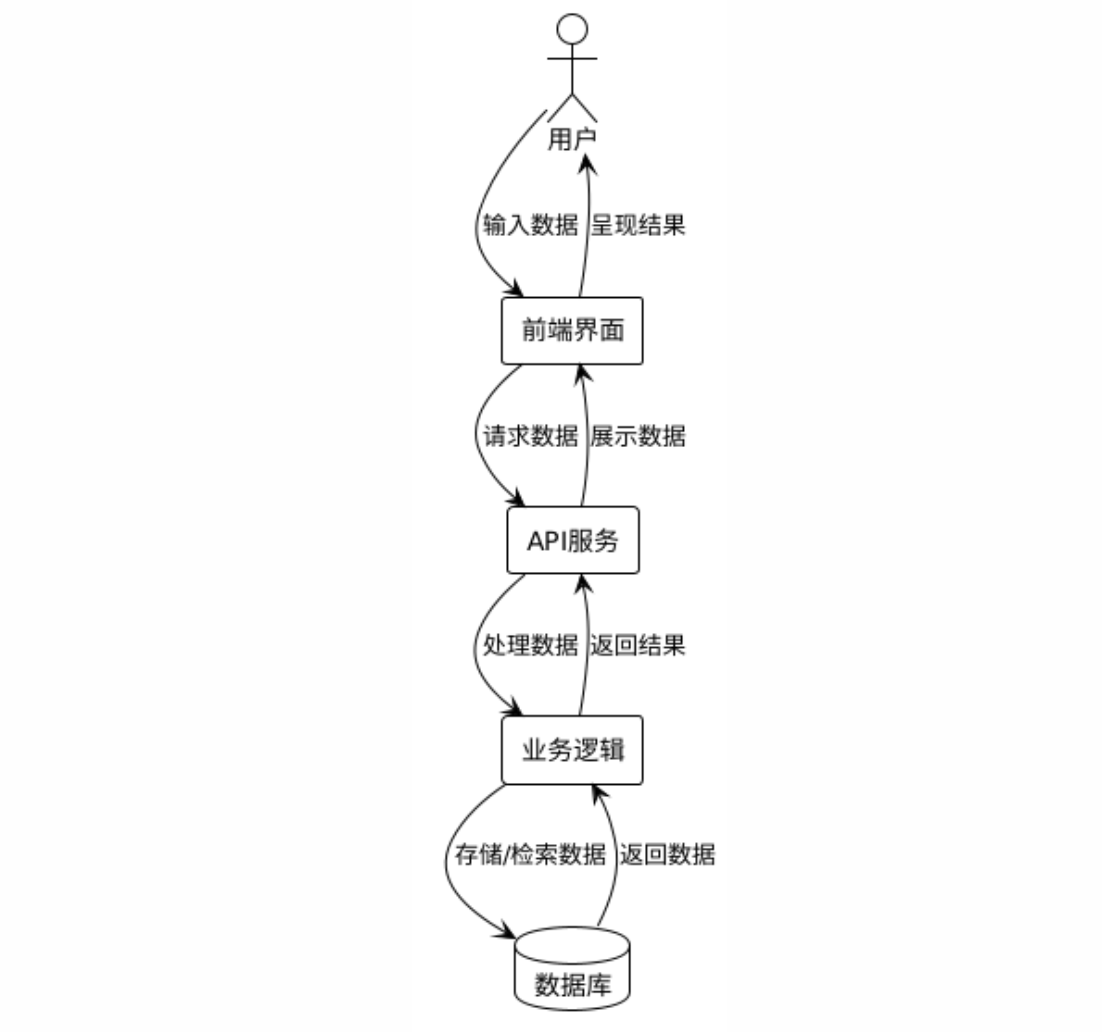
\includegraphics[width=0.75\linewidth]{assets/6.png}
    \caption{数据流图}
    \label{fig:data-flow}
\end{figure}
\section{接口需求}

\subsection{System组与其他组接口概述}

System组作为项目的技术基础设施提供者,需要与UI组、Data组和Analysis组建立明确的接口,确保各组协作顺畅。以下图表展示了System组与其他组的主要接口关系:

\begin{figure}[H]
    \centering
    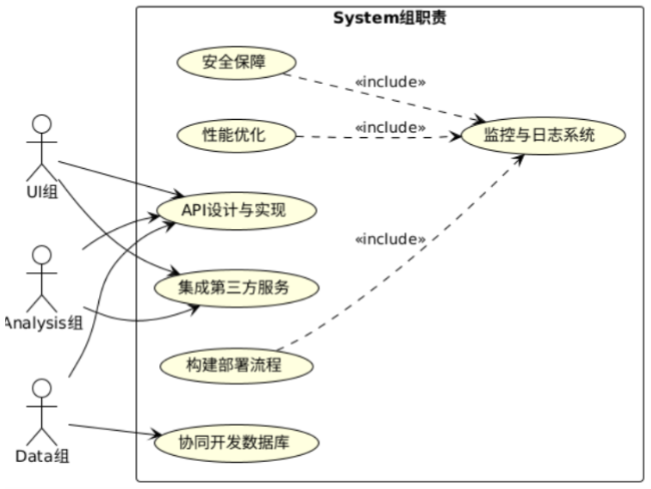
\includegraphics[width=0.8\linewidth]{assets/image2.png}
    \caption{System组与其他组的接口关系图}
    \label{fig:interface-relations}
\end{figure}

\subsection{System组与UI组接口}

System组为UI组提供后端服务支持,两组之间的接口主要体现在API层面。

\subsubsection{API接口规范}

\begin{itemize}
  \item \textbf{接口风格}:RESTful API
  \item \textbf{数据格式}:JSON
  \item \textbf{认证方式}:JWT (JSON Web Token)
  \item \textbf{状态码使用}:遵循HTTP标准状态码
  \item \textbf{版本控制}:URL路径中包含版本号,如/api/v1/users
  \item \textbf{错误处理}:统一的错误响应格式
  \item \textbf{分页机制}:支持limit/offset和cursor分页
\end{itemize}

\subsubsection{核心API接口}

\begin{longtable}{|p{3cm}|p{2.5cm}|p{2.5cm}|p{7cm}|}
\hline
\textbf{接口名称} & \textbf{请求方法} & \textbf{路径} & \textbf{说明} \\
\hline
\endhead
用户认证 & POST & /api/v1/auth/login & UI组调用此接口进行用户登录认证 \\
\hline
获取用户信息 & GET & /api/v1/users/profile & 获取当前登录用户的详细信息 \\
\hline
数据查询 & GET & /api/v1/data & 支持多种查询参数,返回分页数据 \\
\hline
数据操作 & POST/PUT/DELETE & /api/v1/data & 创建、更新、删除数据 \\
\hline
文件上传 & POST & /api/v1/files & 支持多文件上传,返回文件URL \\
\hline
系统配置 & GET & /api/v1/config & 获取UI所需的系统配置参数 \\
\hline
\end{longtable}

\subsubsection{前后端交互流程}

\begin{enumerate}
  \item \textbf{用户认证流程}
  \begin{itemize}
    \item UI组收集用户凭证(用户名/密码)
    \item 调用认证API获取访问令牌
    \item 后续请求携带令牌进行身份验证
  \end{itemize}
  
  \item \textbf{数据交互流程}
  \begin{itemize}
    \item UI组按照API规范构造请求
    \item System组处理请求并返回适当的响应
    \item UI组根据响应更新界面
  \end{itemize}
  
  \item \textbf{错误处理流程}
  \begin{itemize}
    \item System组返回标准错误码和详细错误信息
    \item UI组根据错误类型显示适当的错误提示
  \end{itemize}
\end{enumerate}

\subsection{System组与Data组接口}

System组与Data组在数据库开发和数据处理方面紧密协作,接口设计需要考虑数据访问效率和安全性。

\subsubsection{数据库访问接口}

\begin{itemize}
  \item \textbf{数据访问模式}:Repository模式
  \item \textbf{ORM框架}:提供对象关系映射能力
  \item \textbf{事务支持}:支持分布式事务
  \item \textbf{缓存机制}:多级缓存策略
  \item \textbf{连接池管理}:优化数据库连接资源
\end{itemize}

\subsubsection{主要数据交互场景}

\begin{longtable}{|p{3cm}|p{4cm}|p{8cm}|}
\hline
\textbf{交互场景} & \textbf{接口方法} & \textbf{说明} \\
\hline
\endhead
数据查询 & findById(), findByCondition() & 支持单条记录查询和条件查询,Data组负责SQL优化 \\
\hline
数据写入 & save(), update(), delete() & 提供统一的数据写入接口,System组处理并发控制 \\
\hline
批量操作 & batchInsert(), batchUpdate() & 高性能批量数据处理接口 \\
\hline
数据迁移 & migrateData() & 版本升级时的数据迁移接口 \\
\hline
数据验证 & validate() & 数据业务规则验证,确保数据一致性 \\
\hline
\end{longtable}

\subsubsection{职责分工}

\begin{itemize}
  \item \textbf{Data组职责}:
  \begin{itemize}
    \item 设计数据库结构(表、索引、约束)
    \item 优化数据库查询性能
    \item 编写数据库变更脚本
    \item 管理数据库版本
  \end{itemize}
  
  \item \textbf{System组职责}:
  \begin{itemize}
    \item 实现数据访问层代码
    \item 处理数据业务逻辑
    \item 确保数据访问安全
    \item 实现数据缓存机制
    \item 管理数据库连接资源
  \end{itemize}
\end{itemize}

\subsection{System组与Analysis组接口}

System组为Analysis组提供数据服务和计算资源,支持Analysis组进行各类数据分析。

\subsubsection{数据分析API}

\begin{itemize}
  \item \textbf{数据获取API}:提供结构化数据查询接口
  \item \textbf{数据流API}:支持流式数据处理
  \item \textbf{计算任务API}:支持异步分析任务提交和结果获取
  \item \textbf{结果存储API}:提供分析结果持久化能力
\end{itemize}

\subsubsection{主要交互场景}

\begin{longtable}{|p{3cm}|p{4cm}|p{8cm}|}
\hline
\textbf{交互场景} & \textbf{接口方法} & \textbf{说明} \\
\hline
\endhead
原始数据获取 & fetchRawData() & 获取指定条件的原始数据,支持分页和筛选 \\
\hline
提交分析任务 & submitTask() & 提交异步分析任务,返回任务ID \\
\hline
获取任务状态 & getTaskStatus() & 查询分析任务的执行状态 \\
\hline
获取分析结果 & getTaskResult() & 获取已完成任务的分析结果 \\
\hline
注册数据回调 & registerCallback() & 分析结果生成后自动通知Analysis组 \\
\hline
\end{longtable}

\subsubsection{数据格式规范}

\begin{itemize}
  \item \textbf{输入数据格式}:JSON、CSV或二进制格式
  \item \textbf{元数据描述}:提供数据结构和字段描述
  \item \textbf{输出结果格式}:统一的分析结果格式
  \item \textbf{错误信息格式}:详细的错误码和描述
\end{itemize}

\subsection{跨组协作接口}

某些功能需要多个组共同协作,System组需要提供协调多组工作的接口。

\subsubsection{通知与事件系统}

\begin{itemize}
  \item \textbf{事件发布接口}:System组发布系统事件
  \item \textbf{事件订阅接口}:其他组订阅感兴趣的事件
  \item \textbf{消息队列}:确保事件异步处理不阻塞主流程
  \item \textbf{事件类型}:系统状态变更、任务完成、数据更新等
\end{itemize}

\subsubsection{集成测试接口}

\begin{itemize}
  \item \textbf{测试环境配置}:提供独立测试环境接口
  \item \textbf{测试数据生成}:生成测试数据的接口
  \item \textbf{状态重置}:测试后恢复系统状态的接口
  \item \textbf{模拟接口}:模拟第三方服务的接口
\end{itemize}

\subsection{接口文档与版本管理}

\subsubsection{接口文档规范}

\begin{itemize}
  \item \textbf{文档格式}:采用OpenAPI(Swagger)规范
  \item \textbf{必要字段}:接口URL、请求方法、参数说明、响应格式、错误码
  \item \textbf{示例代码}:各语言的调用示例
  \item \textbf{更新记录}:接口变更历史
\end{itemize}

\subsubsection{接口版本管理}

\begin{itemize}
  \item \textbf{版本命名}:主版本.次版本.修订版本(如1.2.3)
  \item \textbf{兼容性原则}:次版本和修订版本必须向后兼容
  \item \textbf{废弃流程}:接口废弃前需要提前公告,保留过渡期
\end{itemize}

\subsubsection{接口变更管理}

\begin{itemize}
  \item \textbf{变更评审}:重要接口变更需多组评审
  \item \textbf{变更通知}:接口变更前通知相关方
  \item \textbf{变更测试}:新接口必须通过自动化测试
  \item \textbf{回滚机制}:接口上线后发现问题可快速回滚
\end{itemize}

\section{约束与假设}

\subsection{技术约束}

\begin{enumerate}
  \item 系统应使用现代Web技术开发
  \item 数据库选择应考虑性能和可扩展性
  \item 系统应支持主流浏览器
  \item 开发应遵循安全编码规范
\end{enumerate}

\subsection{业务约束}

\begin{enumerate}
  \item 系统应符合相关行业法规和标准
  \item 数据处理应遵循数据保护原则
  \item 系统功能应与现有业务流程兼容
\end{enumerate}

\subsection{假设条件}

\begin{enumerate}
  \item 用户具备基本的计算机操作技能
  \item 系统运行环境满足最低硬件要求
  \item 网络连接稳定可靠
  \item 用户数据可从现有系统迁移
\end{enumerate}

\section{验收标准}

\subsection{功能验收标准}

系统验收应满足以下功能标准:

\begin{enumerate}
  \item 用户可完成所有核心业务流程
  \item 数据处理结果准确无误
  \item 报表生成功能正常运行
  \item 系统管理功能完备可用
\end{enumerate}

\subsection{非功能验收标准}

系统还应满足以下非功能标准:

\begin{enumerate}
  \item 系统响应时间满足性能需求
  \item 安全测试无严重漏洞
  \item 系统可靠性测试通过
  \item 用户界面符合可用性原则
\end{enumerate}

\section{附录}

\subsection{术语表}

\begin{longtable}{|p{3cm}|p{12cm}|}
\hline
\textbf{术语} & \textbf{定义} \\
\hline
\endhead
API & 应用程序编程接口(Application Programming Interface) \\
\hline
UI & 用户界面(User Interface) \\
\hline
ETL & 提取、转换、加载(Extract, Transform, Load) \\
\hline
CI/CD & 持续集成/持续部署(Continuous Integration/Continuous Deployment) \\
\hline
RESTful & 表现层状态转移(Representational State Transfer)架构风格的API设计原则 \\
\hline
\end{longtable}

\subsection{用例关系说明}

\begin{itemize}
  \item \textbf{包含关系(<<include>>)}:表示一个基础用例被包含在另一个用例中,是必须执行的部分
  \item \textbf{扩展关系(<<extend>>)}:表示一个用例在特定条件下扩展另一个用例的行为
  \item \textbf{使用关系}:表示角色使用某个用例提供的功能
  \item \textbf{参与关系}:表示角色参与某个用例的定义或讨论,但不是主要实施者
\end{itemize}

\subsection{修订历史}

\begin{table}[htbp]
\centering
\begin{tabular}{llll}
\toprule
\textbf{版本} & \textbf{日期} & \textbf{修订人} & \textbf{修订内容} \\
\midrule
1.0 & 2025年3月31日 & 蔡旭 & 文档初稿 \\
\bottomrule
\end{tabular}
\caption{文档修订历史}
\end{table}

\end{document} 